\chapter{Resultats}
\label{c:Resultats}

Un cop finalitzada la recerca, passem a la part pràctica. Tal com vam indicar als objectius, el nostre principal propòsit era construir una xarxa neuronal de tipus regressió, que analitza les dades disponibles i genera una predicció numèrica contínua. La nostra ambició ens va fer anar una mica més enllà i construir dues xarxes neuronals diferents com a part de la nostra pràctica. En aquest capítol mostrarem els resultats que hem aconseguit en aquest TR.

\section{Xarxa neuronal de regressió}\label{sec:op}

Una xarxa neuronal de regressió, a diferència d’altres tipus de xarxes, té una sortida lineal que permet predir un valor numèric continu. Aquestes xarxes necessiten un conjunt de dades ampli i ben estructurat perquè puguin aprendre les relacions entre les variables d’entrada i generar prediccions fiables.

A continuació es mostra un esquema representatiu d’una xarxa neuronal de regressió:

\begin{figure}[h!]
\centering
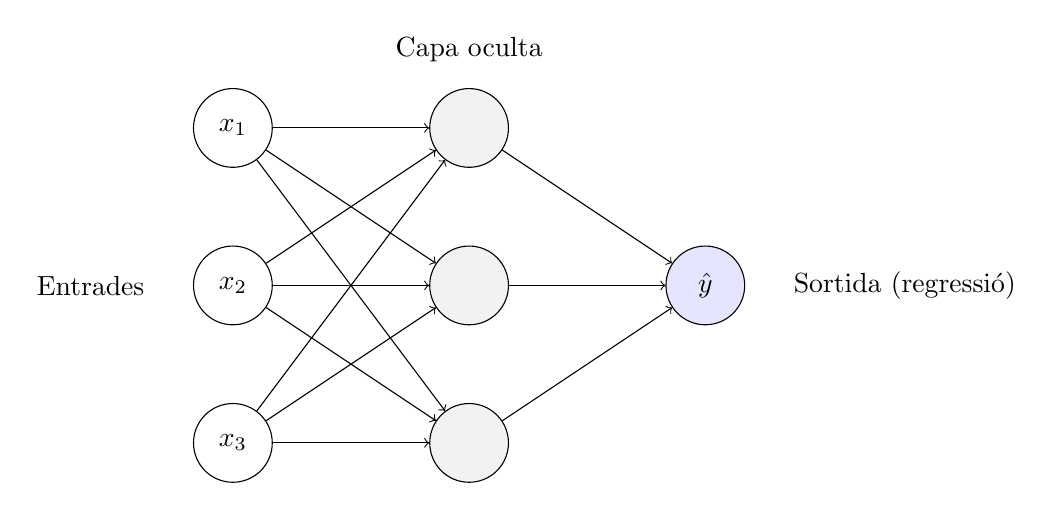
\begin{tikzpicture}[scale=1, transform shape]


\node[circle, draw, minimum size=1cm] (I1) at (0,2) {$x_1$};
\node[circle, draw, minimum size=1cm] (I2) at (0,0) {$x_2$};
\node[circle, draw, minimum size=1cm] (I3) at (0,-2) {$x_3$};


\node[circle, draw, fill=gray!10, minimum size=1cm] (H1) at (3,2) {};
\node[circle, draw, fill=gray!10, minimum size=1cm] (H2) at (3,0) {};
\node[circle, draw, fill=gray!10, minimum size=1cm] (H3) at (3,-2) {};


\node[circle, draw, fill=blue!10, minimum size=1cm] (O1) at (6,0) {$\hat{y}$};


\foreach \i in {1,2,3}
\foreach \h in {1,2,3}
\draw[->] (I\i) -- (H\h);


\foreach \h in {1,2,3}
\draw[->] (H\h) -- (O1);


\node[left] at (-1,0) {Entrades};
\node at (3,3) {Capa oculta};
\node[right] at (7,0) {Sortida (regressió)};

\end{tikzpicture}
\caption{Esquema d’una xarxa neuronal de regressió}
\end{figure}

Abans de crear la xarxa neuronal, vam definir que prediria exactament: les notes finals de matemàtiques dels alumnes. Les dades es recolliren mitjançant un formulari amb les següents preguntes:

\begin{enumerate}
    \item Realització de deures
    \item Hores d’estudi setmanals
    \item Hores de secció
    \item Interès en la matèria
    \item Nota del segon trimestre
    \item Nota del tercer trimestre
    \item Nota final
\end{enumerate}

D’aquesta manera, la xarxa neuronal aprendrà a predir les notes dels alumnes comprenent la relació entre les dades d’entrada i el resultat final.

Per recollir les respostes vam utilitzar Google Drive per crear el formulari i el vam compartir en diversos grups de WhatsApp de batxillerat. Finalment, vam obtenir 18 respostes, tal com es mostra a la imatge següent:

\begin{figure}[h!]
\centering
\includegraphics[width=1\textwidth]{./figures/Formulari.png}
\caption{Resposta a una de les preguntes del formulari}
\end{figure}

Un cop recopilades les dades necessàries, vam començar la construcció de la xarxa neuronal.

\section{Xarxa Neuronal amb llenguatge de programació}\label{sec:10}
En aquest apartat explicarem pas a pas la creació de la nostra xarxa neuronal de regressió amb un llenguatge de programació.

\subsection{De Celcius a Fahrenheit}

Abans de començar a treballar amb la xarxa neuronal definitiva, vàrem crear una de més simple per entendre millor com funciona una xarxa neuronal de regressió. En aquest cas, vaig triar un transformador d’unitats de temperatura, de Celsius (unitat basada en el punt de fusió de l’aigua) a Fahrenheit (sistema basat en els punts d’ebullició i congelació de l’aigua). Aquesta xarxa es va desenvolupar amb el llenguatge de programació Python. Una explicació detallada es pot trobar a l'apèndix~\ref{a:CelsiusFahrenheit}:~\nameref{a:CelsiusFahrenheit}.


\subsection{Predicció de les notes finals de matemàtiques}

Un cop desenvolupada la xarxa neuronal de Celsius a Fahrenheit, ja podem crear la xarxa neuronal que ens havíem proposat. Per començar hem d'importar els frameworks i les biblioteques necessàries: \texttt{numpy}, \texttt{TensorFlow}, \texttt{matplotlib}, \texttt{MinMaxScaler}, \texttt{random} i \texttt{os}.

\begin{itemize}
\item \textbf{MinMaxScaler:} eina de la llibreria \texttt{sklearn} que normalitza les dades i les converteix dins del rang $[0,1]$, facilitant que la xarxa neuronal entengui les relacions numèriques.
\item \textbf{random:} llibreria bàsica de Python que genera i selecciona nombres aleatoris.
\item \textbf{os:} llibreria estàndard de Python que permet treballar amb el sistema operatiu.
\end{itemize}

\begin{figure}[h!]
\centering
\includegraphics[width=0.5\textwidth]{./figures/21.png}
\caption{Biblioteques i frameworks utilitzats}
\end{figure}

A diferència de la xarxa anterior, cal fixar els resultats de la predicció per garantir que les notes finals siguin reproducibles. Amb \texttt{random} podríem seleccionar qualsevol nombre, però per assegurar la coherència assignem la llavor (\texttt{seed}) amb el valor 42. Així, la xarxa sempre s’inicialitzarà amb els mateixos pesos i biaixos.

També es controla l’aleatorietat de les diferents llibreries: \texttt{NumPy}, \texttt{TensorFlow}, \texttt{random}, i s'estableix el valor del hash de Python amb \texttt{os}.

Control de l’aleatorietat:
\begin{itemize}
\item \textbf{Llavor:} \texttt{seed = 42}
\item \textbf{NumPy:} \texttt{np.random.seed(seed)}
\item \textbf{TensorFlow:} \texttt{tf.random.set\_seed(seed)}
\item \textbf{random:} \texttt{random.seed(seed)}
\item \textbf{Python:} \texttt{os.environ["PYTHONHASHSEED"] = str(seed)}
\end{itemize}

\begin{figure}[h!]
\centering
\includegraphics[width=0.5\textwidth]{./figures/22.png}
\caption{Definició dels resultats de les prediccions}
\end{figure}

Un cop fixats els pesos i biaixos, s'emmagatzemen les dades per a l’entrenament. Les dades d’entrada es representen amb \texttt{X}, amb l’ordre de variables següent:

\begin{enumerate}
\item Realització de deures
\item Hores d’estudi setmanals
\item Hores de secció
\item Interès en la matèria
\item Nota del segon trimestre
\item Nota del tercer trimestre
\end{enumerate}

Definim \texttt{X = np.array([])}, creant així una llista que anirem omplint amb les dades del formulari. L’estructura ha de ser sempre \texttt{[x1, x2, x3, x4, x5, x6]} amb \texttt{dtype=float} ja que hem de treballar amb nombres decimals.

La sortida, \texttt{y}, tindrà una sola columna amb els valors de les notes recollides al formulari.

\begin{figure}[h!]
\centering
\includegraphics[width=0.7\textwidth]{./figures/23.png}
\caption{Emmagatzematge de les dades}
\end{figure}

La normalització és crucial perquè la xarxa entengui millor les relacions entre les dades, ja que els valors poden variar molt (hores d’estudi, notes, etc.). Per això utilitzem \texttt{MinMaxScaler} tant per \texttt{X} com per \texttt{y}.

\begin{itemize}
\item Creem l’escalador amb \texttt{scaler = MinMaxScaler()}
\item Normalitzem \texttt{X} amb \texttt{X\_scaled = scaler.fit\_transform(X)}
\item Normalitzem \texttt{y} amb \texttt{scaler\_y} i \texttt{y\_scaled = scaler\_y.fit\_transform(y.reshape(-1,1))}
\end{itemize}

\begin{figure}[H]
\centering
\includegraphics[width=0.5\textwidth]{./figures/24.png}
\caption{Normalització de les dades}
\end{figure}

\begin{figure}[h!]
\centering
\includegraphics[width=0.3\textwidth]{./figures/25.png}
\caption{Normalització Min-Max\cite{Min-Max}}
\end{figure}

A continuació, definim l’estructura de la xarxa neuronal amb un model seqüencial:

\begin{itemize}
\item \textbf{Primera capa oculta:}\\ \texttt{tf.keras.layers.Dense(32, activation="relu", input\_shape=[6])}
32 neurones amb funció d’activació ReLU. L’entrada té 6 característiques corresponents a \texttt{X}.
\item \textbf{Segona capa oculta:}\\ \texttt{tf.keras.layers.Dense(16, activation="relu")}
16 neurones amb ReLU. L’entrada es dedueix automàticament de la capa anterior.
\item \textbf{Capa de sortida:}\\ \texttt{tf.keras.layers.Dense(1)}
Una sola neurona per obtenir la predicció de la nota final. No s’aplica l'activació per mantenir la funció lineal.
\end{itemize}

\begin{figure}[h!]
\centering
\includegraphics[width=0.7\textwidth]{./figures/26.png}
\caption{Estructura de la xarxa neuronal}
\end{figure}

Compilació del model amb \texttt{.compile()}:

\begin{itemize}
\item \textbf{Optimitzador:} \texttt{tf.keras.optimizers.Adam(0.01)}
Ajusta automàticament la taxa d’aprenentatge dels pesos.
\item \textbf{Funció de pèrdua:} \texttt{"mean\_squared\_error"}
Penalitza més fortament els errors grans, millorant la precisió de la predicció.
\item \textbf{Mètrica:} \texttt{["mae"]}
Monitoritza l’error absolut mitjà entre prediccions i valors reals.
\end{itemize}

\begin{figure}[H]
\centering
\includegraphics[width=0.5\textwidth]{./figures/27.png}
\caption{Configuració de la xarxa}
\end{figure}

Entrenament del model amb \texttt{.fit()} utilitzant \texttt{X\_scaled} i \texttt{y\_scaled} durant 400 èpoques, amb \texttt{verbose=1} per mostrar el progrés i l’error per època.

\begin{figure}[H]
\centering
\includegraphics[width=0.7\textwidth]{./figures/28.png}
\caption{Entrenament de la xarxa i corba de pèrdua}
\end{figure}

Per tal predir una nova mostra:
\begin{itemize}
\item Normalització de l’entrada: \texttt{nou\_entrada\_scaled = scaler.transform(nou\_entrada)}
\item Predicció amb la xarxa: \texttt{prediccio = model.predict(nou\_entrada\_scaled)}
\item Transformació inversa: \texttt{prediccio\_real = scaler\_y.inverse\_transform(prediccio)}
\item Mostra del resultat: \texttt{print("Nota prevista:", round(prediccio\_real[0][0],2))}
\end{itemize}

\begin{figure}[h!]
\centering
\includegraphics[width=0.7\textwidth]{./figures/29.png}
\caption{Resultat final i ajustaments}
\end{figure}

% \begin{figure}[h!]
% \centering
% \includegraphics[width=0.5\textwidth]{./figures/27.png}
% \caption{Configuració de la xarxa}
% \end{figure}

% Entrenament del model amb \texttt{.fit()} utilitzant \texttt{X\_scaled} i \texttt{y\_scaled} durant 400 èpoques, amb \texttt{verbose=1} per mostrar el progrés i l’error per època.
%
% \begin{figure}[h!]
% \centering
% \includegraphics[width=0.7\textwidth]{./figures/28.png}
% \caption{Entrenament de la xarxa i corba de pèrdua}
% \end{figure}
%
% Per predir una nova mostra:
%
% \begin{itemize}
% \item Normalització de l’entrada: \texttt{nou\_entrada\_scaled = scaler.transform(nou\_entrada)}
% \item Predicció amb la xarxa: \texttt{prediccio = model.predict(nou\_entrada\_scaled)}
% \item Transformació inversa: \texttt{prediccio\_real = scaler\_y.inverse\_transform(prediccio)}
% \item Mostra del resultat: \texttt{print("Nota prevista:", round(prediccio\_real[0][0],2))}
% \end{itemize}
%
% \begin{figure}[H]
% \centering
% \includegraphics[width=0.5\textwidth]{./figures/29.png}
% \caption{Resultat final i ajustaments}
% \end{figure}

\section{Xarxa Neuronal amb full de càlcul}\label{sec:11}
En aquest apartat continuarem amb la xarxa neuronal de regressió però aquesta vegada utilitzarem un full de càlcul.
L'estructura que utilitzarem per a aquesta pràctica serà la del perceptró.

\begin{figure}[h!]
    \centering
    \includegraphics[width=0.75\textwidth]{./figures/perceptro.png}
    \caption{Estructura del perceptró.~\cite{Img_perceptro}}
\end{figure}

Ara començarem la pràctica ordenant les dades de cada alumne del formulari en el full de càlculs.

\begin{figure}[h!]
    \centering
    \includegraphics[width=0.9\textwidth]{./figures/Dades.png}
    \caption{Dades dels alumnes en el full de càlcul}
\end{figure}

Una vegada he ordenat tota la informació, he decidit representar els valors d'entrada d'una forma més senzilla d'entendre i curta, anomenant-los $xi$.
\begin{itemize}
 \item \textbf {Realització dels deures:} X1
 \item \textbf {Hores d'estudi:} X2
 \item \textbf {Hores de son:} X3
 \item \textbf {Interès en la matèria:} X4
 \item \textbf {Notes del segon trimestre:} X5
 \item \textbf {Notes del tercer trimestre:} X6
 \item \textbf {Nota final:} Y
\end{itemize}

Aquesta representació queda així:

\begin{figure}[h!]
    \centering
    \includegraphics[width=0.9\textwidth]{./figures/Dades_resumides.png}
    \caption{Taula resumida}
\end{figure}

L'entrada ``Realització de deures'' és una dada binària que només pot prendre valors 0 o 1.
\subsection{Normalització de dades}\label{subsec:24}
Abans de continuar, recordar què és la normalització de dades.
La normalització de dades és una tècnica de processament que consisteix a transformar dades de diferents escales a una escala comuna, això facilita la comparació i l'anàlisi de la xarxa neuronal i millora el seu rendiment. En el nostre cas, tenim dades binàries i dades ordinàries que poden prendre qualsevol valor, aquest desequilibri afecta els càlculs posteriors si no es resol.

Per aquesta raó, convertirem totes les dades en valors d'entre 0 i 1. Aquest procés implica calcular la mitjana de les dades i la desviació estàndard de cada variable. Per això utilitzant la fórmula següent:
$$z = \frac{x - \mu}{\sigma}$$
\begin{center}
    $z$ és el valor normalitzat\\
    $x$ és el valor original\\
    $\mu$ és la mitjana\\
    $\sigma$ és la desviació típica
\end{center}


Aquests càlculs són fàcils d'obtenir amb les funcions que ens proporciona el full de càlcul.

\begin{figure}[H]
    \centering
    \includegraphics[width=1\textwidth]{./figures/Dades_normalitzades.png}
    \caption{Taula resumida}
\end{figure}

\subsection{Els paràmetres del model}
Ara que ja tenim totes les dades preparades, hem d'assignar a cada variable X el seu pes per determinar la seva importància en la predicció final. Al començament de l'entrenament, assignarem a tots els valors d'entrada el mateix pes, ja que es corregiran lentament durant l'entrenament.
També hem d'afegir el biaix, que és la constant que ajuda a millorar l'ajust de les prediccions.

\begin{figure}[h!]
    \centering
    \includegraphics[width=0.7\textwidth]{./figures/Pesos.png}
    \caption{Taula dels pesos}
    \label{f:pesos}
\end{figure}

A la figura~\ref{f:pesos}, podem observar com ha quedat la taula després d'afegir els pesos als valors d'entrada, cal afegir 6 columnes de pesos respecte a les 6 entrades i una columna més pel biaix.

\subsection{Funció d'error del model}
Fins ara, ja tenim les dades d'entrada normalitzades i els seus respectius pesos inicials assignats, ara podem aplicar la fórmula que s'utilitza en les xarxes neuronals per calcular la predicció temporal de la nota final. Hem de recordar que la fórmula és:
$$\sum w_i x_i + \text{biaix}$$
Després d'aplicar la fórmula, obtindrem la predicció de la nota final, tal com es veu a la figura~\ref{f:prediccio}.

\begin{figure}[h!]
    \centering
    \includegraphics[width=1\textwidth]{./figures/Predicció.png}
    \caption{Prediccions del model}
    \label{f:prediccio}
 \end{figure}

Hem de recordar que els valors de la predicció són erronis, ja que els pesos que hem assignat són aleatoris. Per aquesta raó, el següent pas de la pràctica és entrenar el nostre model per millorar els paràmetres. Per dur això, haurem d'aplicar un procés d'optimització per ajustar aquests paràmetres. En aquest cas utilitzarem l'algoritme gradient descendent.

Començarem afegint més columnes en el nostre full en la nostra taula. Si restem els valors de la predicció ($Y$) amb els valors reals ($y$) obtindrem la diferència entre la nota dels alumnes i les notes predictives.

\begin{figure}[h!]
    \centering
    \includegraphics[width=0.3\textwidth]{./figures/Errors.png}
    \caption{Erros de la predicció}
    \label{f:errors}
\end{figure}

Es pot veure a~\ref{f:errors} dues columnes addicionals, la columna ``error'' emmagatzema els errors del model i l'altre conté els mateixos errors, però en valor absolut, és a dir, que tots els valors estan en positiu, d'aquesta manera serà més fàcil apreciar la diferència dels errors en les prediccions i els càlculs dels paràmetres.

Després de crear aquestes taules, calcularem la mitjana dels valors que estan en la taula dels errors en positiu, el resultat d'aquesta mitjana ens ajudarà a orientar-nos i determinar si en cada iteració l'error està augmentant o disminuint, com més baix sigui aquest valor, la predicció serà més precisa.

\subsection{Canvis dels paràmetres}
Un cop tenim la funció d'error de la primera predicció, el pas següent és entrenar el model per ajustar els valors dels pesos i del biaix adequadament perquè les següents prediccions siguin més precises.
Per aconseguir això, hem de tenir en compte les dades següents: Quan la diferència de $Y$ respecte a $y$ és més gran, més lluny estaran els pesos dels seus valors ideals. Per tant, hem de trobar la forma de calcular de forma correcta els pesos respecte de la diferència dels valors de la predicció.

Gràcies a la fórmula de la xarxa neuronal sabem que si el valor d'entrada ($X$) és petit, el seu pes ($W$) també ho serà, ja que aquests es multipliquen. Hem de tenir en compte dues coses: La diferència de la predicció final ($Y$) i del valor real ($y$) i el valor d'entrada ($X$) respecte al seu pes ($W$). Per tant, fórmula que utilitzarem per calcular els canvis dels paràmetres serà:
$$\Delta W = (Y_{\text{original}} - Y_{\text{predicció}}) \times X$$
Aquesta fórmula serà la que ens ajudarà a ajustar els paràmetres per tal que la predicció sigui cada cop més precisa. Aplicant aquesta fórmula a cada una de les dades, obtindrem 7 columnes més.

\begin{figure}[h!]
    \centering
    \includegraphics[width=0.9\textwidth]{./figures/Canvis.png}
    \caption{Canvis en els paràmetres}
    \label{f:canvisParametres}
\end{figure}

A la figura~\ref{f:canvisParametres} es pot veure aquestes taules, els canvis del biaix es calculen amb la mateixa fórmula que els pesos, però sense restar-li cap entrada, ja que actua com una entrada constant.
Ara és necessari calcular la mitjana dels canvis dels pesos, les mitjanes obtingudes a partir dels canvis seran uns dels valors que utilitzarem per ajustar els paràmetres.

\subsection{La taxa d'aprenentatge}
Abans de començar a entrenar el model, hem de parlar d'una variable molt important: la taxa d'aprenentatge. Aquesta taxa és un paràmetre que ajusta l'ample dels passos que fem per actualitzar els pesos i el biaix del model, el valor d'aquesta taxa no pot ser molt gran perquè podria dificultar trobar el punt de convergència, ni molt petit perquè ralentitzaria la xarxa.

Normalment, el valor de la taxa d'aprenentatge és 1, però de vegades aquest valor és massa gran i augmentaria l'error del model, si això passa hauríem de reduir el seu valor progressivament fins a un punt on l'error de la xarxa disminueixi significativament.

Finalment, per trobar el valor final dels canvis ajustats dels paràmetres haurem de multiplicar a mitjana dels canvis dels pesos per la taxa d'aprenentatge.

\subsection{Èpoques d'entrenament}
Ja podem començar a entrenar el model, ho farem copiant la mateixa taula que tenim a sota, com es veu a la figura~\ref{f:entrenament}.

\begin{figure}[H]
    \centering
    \includegraphics[width=1\textwidth]{./figures/Etapa_1.png}
    \caption{Èpoques d'entrenament}
    \label{f:entrenament}
\end{figure}

Cada època d'entrenament representa una iteració, podem veure que els paràmetres de la primera època han canviat respecte els de la primera taula, que anomenarem època 0, on aquests paràmetres eren inicialment aleatoris, el valor del primer pes de l'època 1 ($W1$) es calcula sumant el pes de l'època 0 pel valor del canvi ajustat.

Per saber si el model ha millorat, la millor forma de comprovar-ho és fixant-se en la taula dels errors en positiu. Podem veure que aquest valor ha disminuït respecte a l'època anterior, això significa que està millorant.

A partir d'ara hem de fer-ho mateix repetidament fins que el canvi de l'error entre les èpoques siguin molt petits, quan passi això significarà que estem pràcticament en el punt de convergència.%, i és important anant ajustant la taxa d'aprenentatge.

\subsection{Resultats}
En aquest cas, han calgut 8 etapes per arribar al punt de convergència. Hem organitzat els valors de l'error de cada època en una gràfica perquè sigui més fàcil visualitzar els canvis.


\begin{figure}[h!]
    \centering
    \includegraphics[width=0.9\textwidth]{./figures/Gràfica_error.png}
    \caption{Gràfica dels valors d'error en cada època}
    \label{f:errorsEpoca}
\end{figure}


A la figura~\ref{f:errorsEpoca}, podem apreciar que l'error ha disminuït dràsticament entre l'època 0 fins a l'època 4, però després de la cinquena època l'error pràcticament no s'ha mogut, vaig ajustar la taxa d'aprenentatge moltes vegades, però l'error encara baixava molt lentament, fins que va arribar a l'etapa 8. Això vol dir que el model no podia ajustar més els pesos.


\section{Resultats de la xarxa neuronal amb Python}
\begin{comment}
\fbox{\parbox{0.9\linewidth}{\textbf{\emph{
    Hem de tenir en compte que les notes finals dels alumnes estan arrodonides;
    per tant, considerarem que la predicció ha estat encertada si té un marge
    d'error menor a 0,5.
  }}}%
}
\end{comment}
Un cop finalitzada la construcció de la xarxa neuronal, vam avaluar-ne el rendiment, que va assolir una precisió del 93,75\%. Aquest valor l'hem tret considerant correcte totes les prediccions amb un marge d'error menor a 0,5 punts, ja que les notes dels alumnes estan arrodonides. Mitjançant l’ús d’un full de càlcul vam poder organitzar les dades obtingudes estadísticament.

\begin{figure}[h!]
 \centering
 \includegraphics[width=0.9\textwidth]{./figures/Resultats.png}
 \caption{Resultats obtinguts per la xarxa neuronal amb Python}
 \label{f:resultats}
\end{figure}


\section{Resultats de la xarxa neuronal en fulls de càlculs}\label{sec: full de càlcul}
Desprès de finalitzar totes les etapes, els pesos s'han ajustat correctament i, encara que l'error no s'hagi pogut aproximar-se molt al zero absolut, ja és un valor molt petit que podem donar per bo. A la seguent figura podem veure els valors dels pesos finals del model.

\begin{figure}[H]
    \centering
    \includegraphics[width=0.9\textwidth]{./figures/Pesos_finals.png}
    \caption{Pesos finals del model}
\end{figure}

Amb aquests pesos, el model hauria de ser capaç d'obtenir unes prediccions precises respecte a la nota final dels alumnes, per obtenir els valors finals de la predicció, hem de convertir els valors normalitzats de la columna de la predicció de Y de l'última etapa en valors normals, aïllant en la mateixa fòrmula que vam emprar per normalitzar les dades.
$$z = \frac{x - \mu}{\sigma}$$

\begin{figure}[h]
    \centering
    \includegraphics[width=0.8\textwidth]{./figures/Resultat_final.png}
    \caption{Prediccions finals de la pràctica}
    \label{f:resulat_full}
\end{figure}

A la figura~\ref{f:resulat_full}, desprès de desnormalitzar els valors, he organitzat les notes inicials i les prediccions finals en unes taules per visualitzar-los millor, a un costat tenim les notes originals i per l'altre les predictives.
Això ens dona que la xarxa neuronal ha encertat 10 notes de 15, per tant té una precisió aproximada del 66,7 percent.

\section{Comparació resultats Python i Full de càlcul}

A continuació compararem les dues xarxes neuronals determinar quina de les dues és millor:

\begin{itemize}

 \item \textbf{Precisió: } Un dels factors més importants a l'hora de crear una xarxa neuronal predictiva és el seu percentatge d'encert, en aquest cas, la precisió de la xarxa neuronal feta per Python (93,75\%) ha sigut molt més alta que la del full de càlcul (66,7\%)

 \item \textbf{Coneixements previs: } Fer una xarxa neuronal amb Python requereix coneixements de programació, aprendre el llenguatge és indispensable per crear una xarxa neuronal, en canvi, en la xarxa feta amb full de càlcul no ha calgut cap mena de coneixements de programació.

  \item \textbf{Dificultat: } Segons la experiència de cadascun de nosaltres, fer una xarxa neuronal amb full de càlcul és molt més senzill que fer-ho amb Python. No només cal saber programar, a més cal codificar tot el procés de manera manual. En canvi amb el full de câlcul el procés és molt més intuïtiu i mecànic.

  \item \textbf{Temps d'elaboració: } El temps que es requereix en fer una xarxa amb Python depèn de l'habilitat que tinguis en programar, si la persona és àgil i coneix bé el llenguatge pot fer la feina en molt poc temps, mentre que en un full de càlcul, malgrat que les dades i els càlculs s'obtenen automàticament, les etapes es fan manualment, cosa que es torna repetitiva i requereix molt de temps.

  \item \textbf{Visualització: } En una xarxa construida amb un llenguatge de programació està tot automatitzat, la qual cosa, no mostra res de tot el procés que ha elaborat fins al resultat, en canvi, al full de càlcul, passa tot el contrari, es construeix tot manualment, això vol dir que et mostra tots els càlculs intermedis que porten al resultat final, per tant, resulta molt més didâctica.

\end{itemize}

